\subsection{位置族与尺度族}\label{sec:3.5}\index{SI0647@位置尺度族}
在\autoref{sec:3.3}和\autoref{sec:3.4}中，我们讨论了若干常见连续分布族. 本节讨论构造分布族的三种方法. 所得到的族具有易于理解的实际解释，因而适合建模，同时也有方便的数学性质.

这三类族称为位置族、尺度族和位置—尺度族. 每一类族的构造，都是先指定一个pdf，例如$f(x)$，称为该族的标准pdf（standard pdf）. 然后按指定方式变换这个标准pdf，生成族中的所有其他pdf. 我们从关于pdf的一个简单定理开始.\index{SI0651@标准概率密度函数}\semanticindexanchor{651:126}
\sourcepageanchor{127}

\begin{theorem}\label{thm:3.5.1}
设$f(x)$为任意pdf，$\mu$与$\sigma>0$为任意给定常数. 则函数
$$g(x\mid\mu,\sigma)=\frac1\sigma f\left(\frac{x-\mu}\sigma\right)$$
也是pdf.
\end{theorem}
\begin{proof}
为验证这个变换产生了合法的pdf，需要检查：对代入公式的每个$\mu$与$\sigma$值，$(1/\sigma)f((x-\mu)/\sigma)$作为$x$的函数都是pdf. 即须检查它非负且积分为1. 因为$f(x)$是pdf，所以对所有$x$都有$f(x)\ge0$. 于是对所有$x,\mu,\sigma$都有$(1/\sigma)f((x-\mu)/\sigma)\ge0$. 再注意
\begin{align*}
\int_{-\infty}^\infty\frac1\sigma f\left(\frac{x-\mu}\sigma\right)\,dx
&=\int_{-\infty}^\infty f(y)\,dy\qquad\left(\text{令 }y=\frac{x-\mu}\sigma\right)\\
&=1\qquad(\text{因为 }f(y)\text{是pdf}),
\end{align*}
即得所需结论.
\end{proof}
现在转向第一种构造，即位置族的构造.

\begin{definition}\label{def:3.5.2}\index{SI0648@位置参数}
设$f(x)$为任意pdf. 则由参数$\mu$，$-\infty<\mu<\infty$标识的pdf族$f(x-\mu)$，称为以$f(x)$为标准pdf的位置族（location family）；$\mu$称为该族的位置参数（location parameter）.
\end{definition}
为了解引入位置参数$\mu$的效果，考虑\autoref{fig:3.5.1}. 在$x=\mu$处，$f(x-\mu)=f(0)$；在$x=\mu+1$处，$f(x-\mu)=f(1)$；一般地，在$x=\mu+a$处，$f(x-\mu)=f(a)$. 当然，$\mu=0$时$f(x-\mu)$就是$f(x)$. 因此，位置参数$\mu$只把pdf $f(x)$平移，图形形状保持不变，但$f(x)$中原来在$x=0$上方的图上点，在$f(x-\mu)$中位于$x=\mu$上方. 从\autoref{fig:3.5.1}可清楚看出，$f(x)$图形下$x=-1$与$x=2$之间的面积，等于$f(x-\mu)$图形下$x=\mu-1$与$x=\mu+2$之间的面积. 因此，若$X$是pdf为$f(x-\mu)$的随机变量，就可写成
$$P(-1\le X\le2\mid0)=P(\mu-1\le X\le\mu+2\mid\mu),$$
其中等式左边随机变量$X$的pdf为$f(x-0)=f(x)$，右边的pdf为$f(x-\mu)$.

\autoref{sec:3.2}中介绍的若干族，本身就是位置族，或包含位置族作为子族.\footnote{译注：原文此处指向\hyperref[sec:3.2]{第3.2节}，但随后列出的正态、Cauchy和双指数分布均在\autoref{sec:3.3}介绍；原交叉引用疑应为\hyperref[sec:3.3]{第3.3节}.} 例如，若$\sigma>0$是一个指定的已知数，定义
$$f(x)=\frac1{\sqrt{2\pi}\sigma}e^{-x^2/(2\sigma^2)},\qquad-\infty<x<\infty,$$
\begin{figure}[htbp]
\centering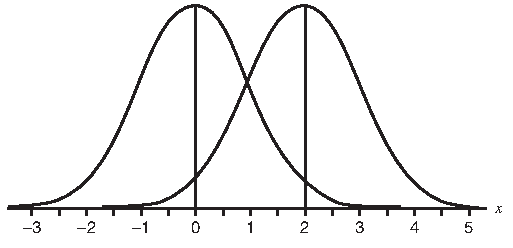
\includegraphics[width=.72\textwidth]{assets/chapter3/fig3-5-1.pdf}
\caption{同一位置族的两个成员：均值为0和2}\label{fig:3.5.1}
\end{figure}
\sourcepageanchor{128}

则以$f(x)$为标准pdf的位置族，就是均值$\mu$未知而方差$\sigma^2$已知的正态分布集合. 为看出这一点，只须验证在上式中以$x-\mu$替换$x$，得到的pdf具有\eqref{eq:3.3.13}定义的形式. 类似地，Cauchy族，以及$\sigma$为指定值、$\mu$为参数的双指数族，都是位置族的例子. 不过，\autoref{def:3.5.2}的关键在于，可以从任意pdf $f(x)$出发，引入位置参数来生成一个pdf族.

若$X$是pdf为$f(x-\mu)$的随机变量，则可表示为$X=Z+\mu$，其中$Z$是pdf为$f(z)$的随机变量. 这个表示是稍后将证明的\autoref{thm:3.5.6}（取$\sigma=1$）的结果. 考察这个表示，可看出何时位置族适合用来对观测变量$X$建模. 下面描述两种情形.

首先，假设一个实验旨在测量某个物理常数$\mu$，例如一种溶液的温度. 但观测中存在测量误差，所以实际观测值$X$为$Z+\mu$，其中$Z$是测量误差. 对这次观测，若$Z>0$，则$X$大于$\mu$；若$Z<0$，则$X$小于$\mu$. 从过去用这个测量装置测量其他溶液的经验中，可能已很清楚随机测量误差的分布. 若该分布的pdf为$f(z)$，则观测值$X$的pdf就是$f(x-\mu)$.

再举一个例子：假设由以往实验已知驾驶员在协调性测试中的反应时间分布. 用随机变量$Z$表示随机选取一位驾驶员的反应时间. 设描述已知分布的$Z$的pdf为$f(z)$. 现在考虑对这个总体“施加处理”. 例如，假设每个人都喝三杯啤酒，会发生什么？可以假定每个人的反应时间都会改变某个未知量$\mu$. （这个非常简单的模型假定每个人的反应时间都改变相同的量$\mu$，可能不是最好的模型. 例如，已知酒精的作用与体重有关，所以较重的人受到啤酒的影响可能较小.）作为思想开放的科学工作者，我们甚至可能允许$\mu<0$，也就是反应时间缩短. 那么，如果我们观察“处理”后一位随机选取的驾驶员的反应时间，这个时间就是$X=Z+\mu$，而$X$的可能分布族由$f(x-\mu)$给出.

若使$f(x)>0$的$x$集合不是整个实数轴，那么使$f(x-\mu)>0$的$x$集合就会依赖于$\mu$. \autoref{ex:3.5.3}说明这一点.

\begin{example}[指数位置族]\label{ex:3.5.3}\index{SI1034@阈值参数}
设$f(x)=e^{-x}$，$x\ge0$；$f(x)=0$，$x<0$. 为构造位置族，以$x-\mu$替换$x$，得到
\begin{align*}
f(x\mid\mu)&=\begin{cases}e^{-(x-\mu)},&x-\mu\ge0,\\0,&x-\mu<0,\end{cases}\\
&=\begin{cases}e^{-(x-\mu)},&x\ge\mu,\\0,&x<\mu.\end{cases}
\end{align*}
不同$\mu$值对应的$f(x\mid\mu)$图形见\autoref{fig:3.5.2}. 与\autoref{fig:3.5.1}一样，图形被平移了. 此时图形的正值部分从$\mu$而非零开始. 若$X$衡量时间，则可能限制$\mu$非负，使每个$\mu$值下$X$都以概率1为正. 在这种模型中，$\mu$表示$X$取值范围的一个界，因而有时称为阈值参数（threshold parameter）.
\end{example}
本节还要讨论的另外两类族是尺度族和位置—尺度族.

\begin{definition}\label{def:3.5.4}\index{SI0650@尺度参数}
设$f(x)$为任意pdf. 对任意$\sigma>0$，由参数$\sigma$标识的pdf族$(1/\sigma)f(x/\sigma)$，称为以$f(x)$为标准pdf的尺度族（scale family），$\sigma$称为该族的尺度参数.
\end{definition}
引入尺度参数$\sigma$的效果是拉伸（$\sigma>1$）或压缩（$\sigma<1$）$f(x)$的图形，同时保持图形的基本形状不变. \autoref{fig:3.5.3}说明了这一点.
\sourcepageanchor{129}

\begin{figure}[htbp]
\centering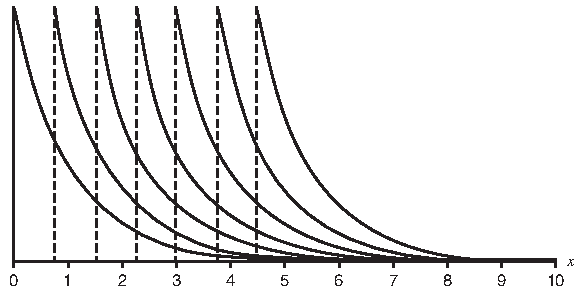
\includegraphics[width=.72\textwidth]{assets/chapter3/fig3-5-2.pdf}
\caption{指数位置密度}\label{fig:3.5.2}
\end{figure}
\begin{figure}[htbp]
\centering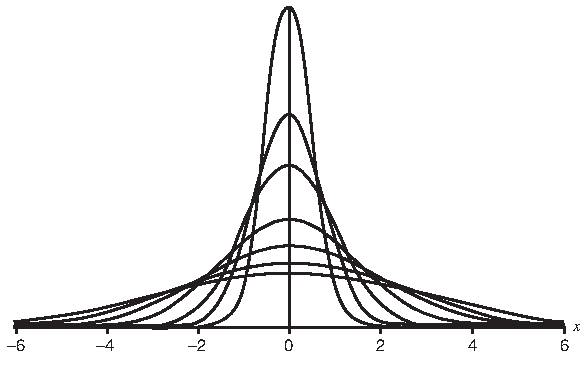
\includegraphics[width=.72\textwidth]{assets/chapter3/fig3-5-3.pdf}
\caption{同一尺度族的成员}\label{fig:3.5.3}
\end{figure}
使用尺度参数时，$f(x)$通常或者关于0对称，或者仅在$x>0$时为正. 此时拉伸或者关于0对称，或者仅沿正方向进行. 但在定义中，任意pdf都可作为标准pdf.

\autoref{sec:3.3}介绍的若干族，本身是尺度族，或含有尺度族作为子族. 这些包括：$\alpha$固定而$\beta$为尺度参数的Gamma族；$\mu=0$而$\sigma$为尺度参数的正态族；指数族；以及$\mu=0$而$\sigma$为尺度参数的双指数族. 在每种情形中，令尺度参数等于1，就得到标准pdf. 然后可证明该族的所有其他成员都具有\autoref{def:3.5.4}中的形式.

\begin{definition}\label{def:3.5.5}\index{SI0648@位置参数}\index{SI0651@标准概率密度函数}
设$f(x)$为任意pdf. 对任意$\mu$，$-\infty<\mu<\infty$，及任意$\sigma>0$，由参数$(\mu,\sigma)$标识的pdf族$(1/\sigma)f((x-\mu)/\sigma)$，称为以$f(x)$为标准pdf的位置—尺度族；$\mu$称为位置参数，$\sigma$称为尺度参数.
\end{definition}
同时引入位置参数和尺度参数的效果是：先像尺度参数那样拉伸（$\sigma>1$）或压缩（$\sigma<1$）图形，再平移图形，使原先在0上方的点现在位于$\mu$上方. \autoref{fig:3.5.4}展示了$f(x)$的这种变换. 正态族和双指数族都是位置—尺度族的例子. \autoref{exercise:3.39}把Cauchy族作为位置—尺度族来讨论.

下面的定理把用于定义位置—尺度族的pdf $f(x)$变换，与pdf为$f(z)$的随机变量$Z$的变换联系起来.
\sourcepageanchor{130}

\begin{figure}[htbp]
\centering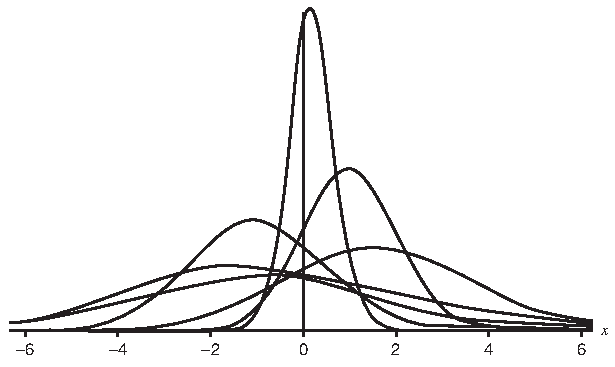
\includegraphics[width=.72\textwidth]{assets/chapter3/fig3-5-4.pdf}
\caption{同一位置—尺度族的成员}\label{fig:3.5.4}
\end{figure}
如前面讨论位置族时所述，用$Z$表示是一种有用的数学工具，也能帮助理解何时位置—尺度族适合建模. 在\autoref{thm:3.5.6}中令$\sigma=1$，得到（仅含）位置族的结果；令$\mu=0$，得到（仅含）尺度族的结果.

\begin{theorem}\label{thm:3.5.6}
设$f(\cdot)$为任意pdf，$\mu$为任意实数，$\sigma$为任意正实数. 则$X$是pdf为$(1/\sigma)f((x-\mu)/\sigma)$的随机变量，当且仅当存在pdf为$f(z)$的随机变量$Z$，使$X=\sigma Z+\mu$.
\end{theorem}
\begin{proof}
为证明“如果”部分，定义$g(z)=\sigma z+\mu$. 则$X=g(Z)$，$g$为单调函数，$g^{-1}(x)=(x-\mu)/\sigma$，且$|(d/dx)g^{-1}(x)|=1/\sigma$. 因此，由\autoref{thm:2.1.5}，$X$的pdf为
$$f_X(x)=f_Z(g^{-1}(x))\left|\frac d{dx}g^{-1}(x)\right|=f\left(\frac{x-\mu}\sigma\right)\frac1\sigma.$$
为证明“仅当”部分，定义$g(x)=(x-\mu)/\sigma$，令$Z=g(X)$. 再次应用\autoref{thm:2.1.5}，有$g^{-1}(z)=\sigma z+\mu$，$|(d/dz)g^{-1}(z)|=\sigma$，且$Z$的pdf为
$$f_Z(z)=f_X(g^{-1}(z))\left|\frac d{dz}g^{-1}(z)\right|=\frac1\sigma f\left(\frac{(\sigma z+\mu)-\mu}\sigma\right)\sigma=f(z).$$
此外，
$$\sigma Z+\mu=\sigma g(X)+\mu=\sigma\left(\frac{X-\mu}\sigma\right)+\mu=X.$$
\end{proof}
从\autoref{thm:3.5.6}可以提取出一个重要事实：随机变量$Z=(X-\mu)/\sigma$具有pdf
\footnote{译注：原式最右端写作$f(x)$，但由左边的自变量及本段定义，应为$f(z)$. 这里保留原式并注明.}
$$f_Z(z)=\frac11f\left(\frac{z-0}1\right)=f(x).$$

也就是说，$Z$的分布是位置—尺度族中对应于$\mu=0,\sigma=1$的成员. 对正态族这一特殊情形，我们已在\autoref{sec:3.3}证明过这一点.

通常可先对pdf为$f(z)$的“标准”随机变量$Z$进行计算，再容易地导出pdf为$(1/\sigma)f((x-\mu)/\sigma)$的随机变量$X$的相应结果. 下面的定理给出一个例子，它推广了\autoref{sec:3.3}中对正态族所作的计算.
\sourcepageanchor{131}

\begin{theorem}\label{thm:3.5.7}
设$Z$是pdf为$f(z)$的随机变量，假定$EZ$与$\operatorname{Var}Z$存在. 若$X$是pdf为$(1/\sigma)f((x-\mu)/\sigma)$的随机变量，则
$$EX=\sigma EZ+\mu\qquad\text{及}\qquad\operatorname{Var}X=\sigma^2\operatorname{Var}Z.$$
特别地，若$EZ=0$且$\operatorname{Var}Z=1$，则$EX=\mu$且$\operatorname{Var}X=\sigma^2$.
\end{theorem}
\begin{proof}
由\autoref{thm:3.5.6}，存在pdf为$f(z)$的随机变量$Z^*$，使$X=\sigma Z^*+\mu$. 所以$EX=\sigma EZ^*+\mu=\sigma EZ+\mu$，且$\operatorname{Var}X=\sigma^2\operatorname{Var}Z^*=\sigma^2\operatorname{Var}Z$.
\end{proof}
对任意均值和方差有限的位置—尺度族，可选择标准pdf $f(z)$，使$EZ=0$且$\operatorname{Var}Z=1$. （证明可以这样选择，留作\autoref{exercise:3.40}.）于是$\mu$和$\sigma^2$就分别可方便地解释为$X$的均值和方差. \autoref{sec:3.3}给出的通常正态族定义就是这种情形. 然而，\autoref{sec:3.3}给出的通常双指数族定义并未作这种选择；那里$\operatorname{Var}Z=2$.

位置—尺度族任一成员的概率都可以用标准变量$Z$计算，因为
$$P(X\le x)=P\left(\frac{X-\mu}\sigma\le\frac{x-\mu}\sigma\right)=P\left(Z\le\frac{x-\mu}\sigma\right).$$
因此，如果标准变量$Z$的$P(Z\le z)$有数表可查或容易计算，就可得到$X$的概率. 用标准正态表计算正态概率就是这方面的例子.
